\chapter{System Architecture}     
        The system architecture organizes the system's necessities into manageable blocks as shown in figure \ref{fig:systemstructure}.
        It is essentially divided into two major components, the Social Routing Client Application \cite{clientapplicationdocs} and the Social Routing Service with a third one being the external services.
        
        The role of the Client Application is to provide an interface which the user can interact with. This component communicates 
        with either the Social Routing Service or external services when required through the HTTP protocol \cite{httponlinedocs}.
        
        The Social Routing Service processes and stores data that the Client Application can use at any time, as long as the user making 
        the requests is authenticated correctly. It receives HTTP requests and exposes it's functionality through the Social Routing API \cite{apidocs}.

        The external API's are used to make some otherwise very difficult operations achievable in a short period of time. The API's
        used will be mentioned inside each of the components's description.   

        \vfill
        \begin{figure}[h]            
            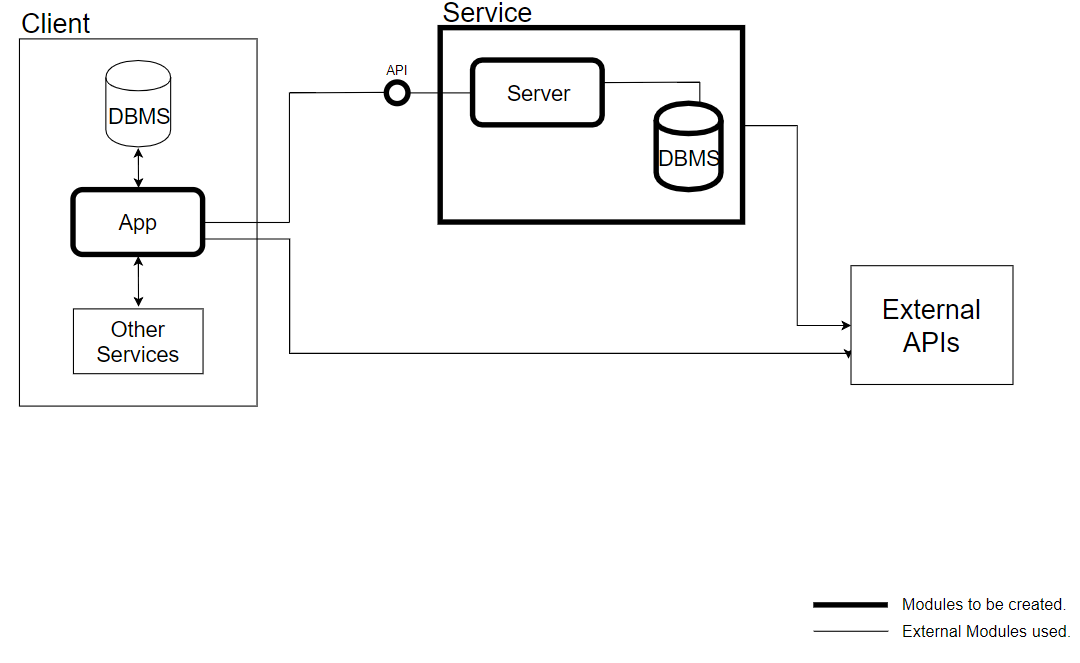
\includegraphics[width=\textwidth]{images/project-structure/system-structure.PNG}
            \caption{System structure.}
            \label{fig:systemstructure}
        \end{figure}  